% !TeX program = pdflatex
% !TeX encoding = UTF-8
% !TeX spellcheck = pt_BR
\documentclass[
  article,
  11pt,
  a4paper,
  english,
  brazil,
  sumario=tradicional]{abntex2}
\usepackage{lmodern}			% Usa a fonte Latin Modern
\usepackage[T1]{fontenc}		% Selecao de codigos de fonte.
\usepackage[utf8]{inputenc}		% Codificacao do documento (conversão automática dos acentos)
\usepackage{indentfirst}		% Indenta o primeiro parágrafo de cada seção.
\usepackage{nomencl} 			% Lista de simbolos
\usepackage{color}				% Controle das cores
\usepackage{graphicx}			% Inclusão de gráficos
\usepackage{microtype} 			% para melhorias de justificação

\usepackage{csquotes}
% ---
% Pacotes de citações
% ---
\usepackage[brazilian,hyperpageref]{backref}	 % Paginas com as citações na bibl
\usepackage[alf]{abntex2cite}	% Citações padrão ABNT
% ---

% ---
% Configurações do pacote backref
% Usado sem a opção hyperpageref de backref
\renewcommand{\backrefpagesname}{Citado na(s) página(s):~}
% Texto padrão antes do número das páginas
\renewcommand{\backref}{}
% Define os textos da citação
\renewcommand*{\backrefalt}[4]{
  \ifcase #1 %
  Nenhuma citação no texto.%
  \or
  Citado na página #2.%
  \else
  Citado #1 vezes nas páginas #2.%
  \fi}%
% ---

% Para fórmulas matemáticas
\usepackage{amsmath}
\usepackage{amssymb}
\usepackage{mathtools}

% Para setas usadas em fórmulas dos grafos
\usepackage{MnSymbol}

% Diretório padrão para figuras
\graphicspath{ {images/} }

% Permite colocar figuras lado a lado ou
% fazer posicionamentos arbitrários
\usepackage[lofdepth,lotdepth]{subfig}

\hypersetup{
  %hidelinks,   % Comente aqui para exibir os links
  colorlinks, % Descomente esse se comentar o de cima
  linkcolor={red!50!black},
  citecolor={blue!50!black},
  urlcolor={blue!80!black}
}

\usepackage[pdftex,dvipsnames,table,xcdraw]{xcolor}

% Para setas usadas em fórmulas dos grafos
\usepackage{MnSymbol}

% ---
% Altera as margens padrões
% ---
\setlrmarginsandblock{3cm}{3cm}{*}
\setulmarginsandblock{3cm}{3cm}{*}
\checkandfixthelayout
% ---

% --- 
% Espaçamentos entre linhas e parágrafos 
% --- 

% O tamanho do parágrafo é dado por:
\setlength{\parindent}{1.3cm}

% Controle do espaçamento entre um parágrafo e outro:
\setlength{\parskip}{0.2cm}  % tente também \onelineskip

% Espaçamento simples
\SingleSpacing

% Titulo e coisas para cabeçalho
\title{Identificação de Fronteiras de Carreiras utilizando Detecção de Comunidades}
\author{Ronie Uliana}

\begin{document}

% Seleciona o idioma do documento (conforme pacotes do babel)
%\selectlanguage{english}
\selectlanguage{brazil}

% Retira espaço extra obsoleto entre as frases.
\frenchspacing

\maketitle

\begin{abstract}
Resumo vai aqui
\end{abstract}

%===================================
\section{Introdução}
%===================================

A trajetória profissional de cada pessoa é bastante particular. Enquanto alguns seguem caminhos estabelecidos, como inúmeros presidentes de empresa que começaram como estagiários, outros trilham por sequências improváveis de ocupações, como o reconhecido chef Alex Atala.

Também os modelos carreiras têm se modificado, e teorias como as das \textit{Carreiras Proteanas} e \textit{Carreiras sem Fronteiras} advogam um distanciamento das carreiras comuns em favor de trajetórias com foco maior no indivíduo~\cite{Bendassolli2009-bg}.

No entanto, o movimento de uma pessoa entre ocupações profissionais não é simples. A capacitação do indivíduo, a atratividade da nova ocupação e o próprio conhecimento que uma transição é possível a tornam mais fácil ou difícil para os profissionais. Quando essa transição é percebida como uma barreira por um número suficiente de pessoas, surge uma \enquote{fronteira de carreira}. Essas fronteiras delimitam um grupo de ocupações onde um indivíduo tem maiores chances de permanecer em sua carreira~\cite{Gunz2007-hr}.

Essa trabalho utiliza os conceitos de fronteiras de carreira, um banco de dados com milhões de experiências profissionais e técnicas de detecção de comunidades em redes para encontrar esses grupos profissionais no mercado de trabalho brasileiro.

A Seção~\ref{sec:carreira} descreve o conceito de fronteira da carreira, a Seção~\ref{sec:mapa} descreve o banco de dados que serve como base para esse pesquisa, a Seção~\ref{sec:comunidades} descreve o algoritmo utilizado para detecção de comunidades. Finalmente, na Seção~\ref{sec:resultados}, os grupos profissionais resultantes são caracterizados e exemplificados. Nessa mesma seção são levantadas questões sobre os resultados que escapam do escopo desse trabalho.

As conexões entre fronteiras de carreira e o algoritmo utilizado para detecção de comunidades são feitas ao final das Seções~\ref{sec:carreira} e~\ref{sec:comunidades}.

%===================================
\section{Carreira e Fronteira} \label{sec:carreira}
%===================================

Segundo~\citeonline{Arthur1989-rn}, carreira é \foreignquote{english}{uma sequência evolutiva da experiência profissional de uma pessoa no tempo}\footnote{No original: \enquote{an evolving sequence of person's work experience over time}.}.

Apesar das discussões sobre as mudanças nos modelos de carreira, passando de um modelo linear e centrado na organização para um modelo centrado no indivíduo, as definições de carreira são frequentemente associadas à progressão ou sequência profissional do indivíduo~\cite{Baruch2004-oy,Sullivan2009-xb,Bendassolli2009-bg}.

Para os fins desse trabalho, define-se carreira como \textit{a sequência de ocupações pela qual um indivíduo passa em sua vida profissional}. Essa definição é similar à de \citeonline{Arthur1989-rn}, porém, limita a abrangência da definição e a torna mais concreta. Isso permite uma análise menos subjetiva, uma vez que ocupações profissionais podem ser extraídas de currículos e analisadas quantitativamente. No entanto, ela se torna mais limitada, já que essa definição exclui aspectos psicológicos ou sociais.

\begin{comment} Ronie, isso é o início de outra argumentação
Em resumo, a argumentação é que uma \enquote{coisa} social é um construto pessoal e subjetivo, mas se torna objetivo quando há um consenso por um número suficiente de pessoas. Essa mesma linha de raciocínio é explorada por \citeonline{Abbott1995-ft} para explicar o surgimento de \enquote{entidades} sociais, como profissões, a partir do reconhecimento das diferenças entre elas por um número crescente de pessoas.
\end{comment}

Essa pesquisa empresta o conceito de \enquote{fronteiras de carreira} (\textit{career boundaries}) como descrito por  \citeonline{Gunz2007-hr} para dar significado ao trabalho.

A fronteira de carreira significa que uma mudança entre ocupações nem sempre pode ser realizada livremente. Por exemplo, um profissional precisa de graduação especializada antes de poder se mover da ocupação de \enquote{Auxiliar de Jardinagem} para \enquote{Médico}, por outro lado, a barreira para mesmo profissional exercer a ocupação de \enquote{Jardineiro} se limita à experiência. É possível perceber que as barreiras não são simétricas, em um momento de crise é mais simples para uma \enquote{Engenheiro} tornar-se um \enquote{Corretor de Imóveis} do que o contrário.

Essas barreiras não se limitam ao conhecimento, quaisquer dificuldades na movimentação podem criar fronteiras. Por exemplo, alguém morando em um grande centro urbano dificilmente exerceria a ocupação de \enquote{Agricultor} sem mover-se para o campo. Um \enquote{Diretor Financeiro} precisaria adequar seu padrão de vida antes de uma transição para uma ocupação com ganhos mais modestos. Uma profissão que está desaparecendo, como \enquote{Contínuo} possui barreiras mais altas do que uma nascendo, como \enquote{Analista de Experiência do Usuário}.

Para os autores, as fronteiras de carreira são subjetivas e pessoais; cada um tem para si quais transições podem ser feitas em sua carreira. No entanto, essas fronteiras se tornam objetivas quando um número suficientemente grande de pessoas possui a mesma compreensão sobre essas transições, a ponto dela ser perceptível em um nível macroscópico.

Dessa maneira, o consenso define as fronteiras de carreira objetivamente quando existe uma quantidade suficiente de pessoas entra em consenso sobre quais são transições incomuns. A fronteira define o grupo, e não o contrário~\cite{Gunz2007-hr}.

Partindo desse pressuposto, a identificação de trajetórias comuns e incomuns é condição suficiente e necessária para a detecção de fronteiras entre carreiras. Suficiente, pois a própria definição de fronteira é dependente da identificação do que são transições \enquote{incomuns}. Necessária, pois não existem fronteiras objetivamente definidas sem o consenso.

%===================================
\section{O Mapa de Carreiras} \label{sec:mapa}
%===================================

O Mapa VAGAS de Carreiras~\cite{VAGAS_Tecnologia2015-yv} é uma rede que resume as transições dos profissionais entre ocupações no mercado de trabalho. Nele, cada nó representa uma ocupação e as conexões representam o número de profissionais que se movimentou entre elas, ou seja, nas suas carreiras, deixaram a ocupação anterior e passaram a trabalhar em uma nova.

\begin{figure}[ht]
  \centering
  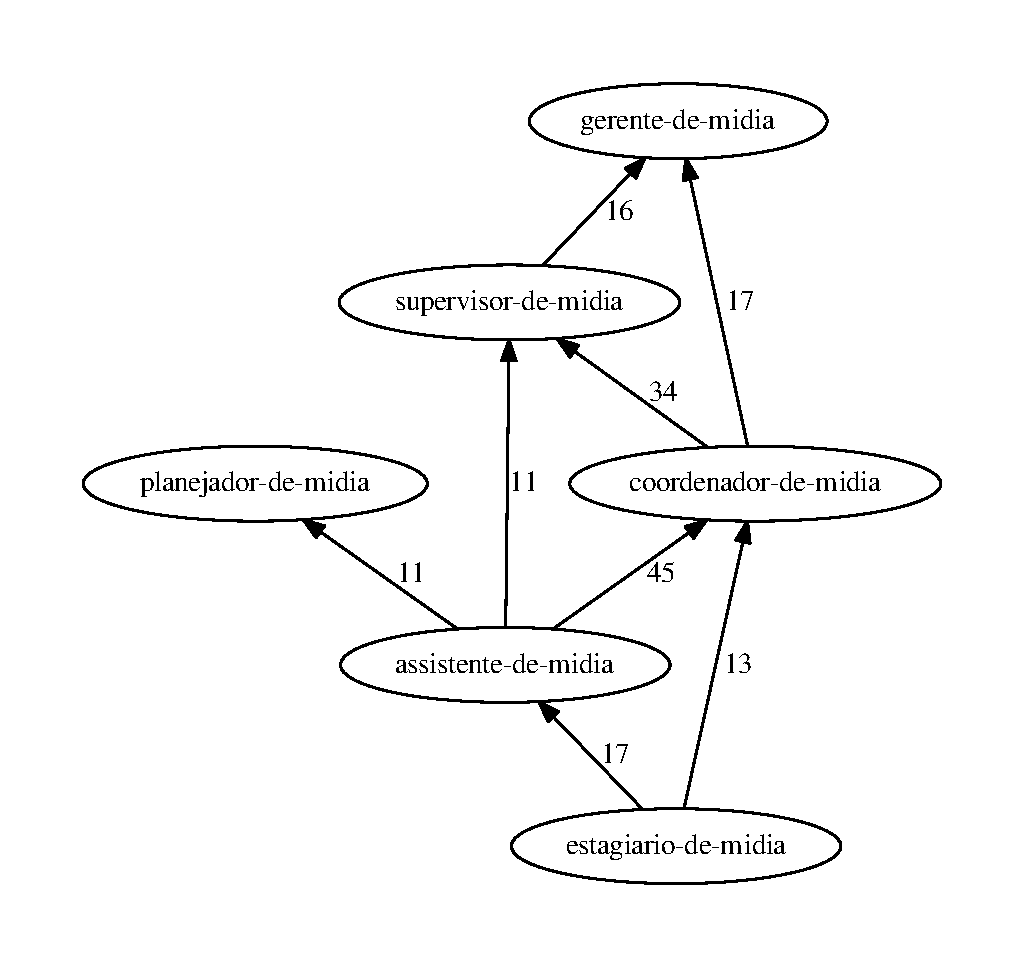
\includegraphics[scale=0.6]{cluster_23.pdf}
  \caption{Parte do Mapa de Carreiras}
  \label{fig:ex-mapa-midia}
\end{figure}

É possível observar parte do Mapa VAGAS de Carreiras (MCar) na Figura~\ref{fig:ex-mapa-midia} com as ocupações relacionadas à profissão de \enquote{mídia}. Nela, por exemplo, 16 pessoas passaram de \enquote{supervisor-de-midia} para a ocupação \enquote{gerente-de-midia} em sua trajetória profissional.

As ocupações no MCar foram definidas a partir de \textit{consenso} nos currículos. Como o título da ocupação é um campo em que o usuário digita livremente, assumiu-se que, se um grupo \enquote{suficientemente grande} de pessoas entra em acordo sobre uma certa nomenclatura, ela representa objetivamente uma ocupação. Essa abordagem é colocada de maneira implícita em ~\citeonline{Abbott1995-ft}, já \citeonline{Gunz2007-hr} a exploram para definir fronteiras de carreiras.

Uma das maiores dificuldades está em se definir o quanto um consenso precisa ser \enquote{suficientemente grande} para de fato existir uma ocupação. Para os fins desse trabalho, esse número foi obtido de forma experimental e empírica. Para isso, procurou-se o número mínimo de repetições exatas na grafia das ocupações de maneira não fossem encontrados erros de digitação recorrentes, ou seja, que das ocupações criadas por consenso, nenhuma fosse resultado de erros frequentes de digitação. Esse número é atualmente 30 repetições, ou 10 transições com exatamente a mesma grafia em ambos os lados da transição.

Para a criação do MCar foram usados os currículos anonimizados de 10 milhões de usuários registrados no site VAGAS.com.br. A seleção de dados, bem como o processamento das informações, seguiu um procedimento conservador. Isso significa que as decisões tomadas em sua construção procuram minimizar os erros decorrentes da qualidade dos dados, mesmo que isso signifique trabalhar com uma quantidade menor de dados.

Da massa de currículos, apenas os atualizados no período entre 2011 e 2016 foram usados. Currículos em duplicação foram removidos usando o CPF como identificador, em caso de duplicação, apenas o currículo mais recente foi considerado. Na impossibilidade de se verificar a duplicação, como por exemplo, na ausência do CPF, o currículo também foi descartado.

Finalmente, algumas informações gerais foram extraídas dos currículos que sobreviveram ao processo acima e o restante das informações foi descartada, incluindo quaisquer maneiras de se identificar a pessoa descrita no currículo.

A informações extraídas são o sexo, último salário, graduação (se existente) ou escolaridade, e a sequência de ocupações pelo qual o profissional passou com o título, descrição e período em que exerceu a ocupação.

O título da ocupação é um dos principais artefatos do MCar, é ele quem fornece a identidade para o nó. Como descrito acima, nos currículos, o título da ocupação é um campo de texto livre, ou seja, o usuário pode digitar o título sem restrições. Se por um lado isso permite a identificação de ocupações de nicho, novas ou que usem jargão de área; também significa que os títulos possuem erros de grafia, variações de gênero (como em \enquote{advogado} e \enquote{advogada} ou \enquote{moto boy} e \enquote{moto girl}), composição de múltiplas ocupações em um mesmo título (como \enquote{caixa / balconista}), abreviações e toda a gama de erros de interpretação possíveis.

As ocupações passam por um corretor ortográfico criado especificamente para esse trabalho, uma vez que um corretor tradicional não é capaz de identificar jargões de área como \enquote{enfermeiranda}, \enquote{rigger} ou \enquote{IRLA}.

Como exemplo, o dicionário do corretor possui cerca de 750 variações ortográficas que são traduzidas para o termo \enquote{auxiliar}, dentre eles, simples erros de omissão como \enquote{uxiliar} até variações mais elaboradas como \enquote{ausciliar} e \enquote{alsilia}.

Após o trabalho de correção ortográfica, os títulos foram agrupados e contados. Especialistas da empresa verificaram os resultados dos maiores grupos para identificar anomalias como os títulos \enquote{sim}, \enquote{não} e \enquote{o mesmo}, essas ocupações foram excluídas do trabalho.

Finalmente, pares de ocupações foram gerados. Por exemplo, um currículo com a sequência de ocupações \enquote{saladeiro} $\to$ \enquote{chapeiro} $\to$ \enquote{cozinheiro} gera os pares \enquote{saladeiro} $\to$ \enquote{chapeiro} e \enquote{chapeiro} $\to$ \enquote{cozinheiro}.

Os pares foram agrupados e sua contagem se torna o peso de cada conexão na rede final. Nesse ponto do processo, cerca de 23 milhões de ocupações dos currículos foram agrupadas em aproximadamente 8 mil ocupações distintas.

Finalmente, os pares de ocupações foram conectado entre si a rede final foi construída e armazenada em um banco de dados de grafo. Um sistema online\footnote{Disponível em \url{http://www.vagas.com.br/mapa-de-carreiras}} disponibiliza as informações publicamente. Apesar de gratuito e de consulta pública, os dados do Mapa VAGAS da Carreira não são de uso livre. A empresa gentilmente cedeu os dados ao pesquisador para esse trabalho.

%===================================
\section{Detecção de Comunidades} \label{sec:comunidades}
%===================================

Uma comunidade é um subgrafo com conexões mais \textit{coesas} entre seus nós do que com nós do restante do grafo. A palavra \enquote{coesão} aqui pode ser interpretada de várias maneiras. Para \citeonline{Ahn2010-uh,Evans2009-lq}, uma comunidade é definida quando o número de conexões internas do subgrafo é maior que o número de conexões que o conecta ao resto do grafo. Para \citeonline{Barabasi2016-rn,Newman2004-jg} a comunidade deve possuir uma densidade de conexões mais alta do que o esperado em uma rede aleatória equivalente. De qualquer forma, para esses autores, o número de conexões é o fator determinante para a identificação da comunidade.

\citeonline{Rosvall2009-sd,Van_Dongen2000-qm}, por sua vez, trabalham a detecção de comunidades como a identificação de fluxos mais frequentes na rede. Assumindo que uma conexão representa um fluxo, comunidades possuem fluxo maior entre seus nós do que com nós fora da comunidade.

Essas abordagens distintas são aplicáveis a cenários diferentes. A densidade de conexões é mais adequada em redes onde a estrutura é importante, como por exemplo, em uma rede social. Já em redes que representam fluxos, com circuitos ou redes de transporte, a segunda abordagem é mais atraente~\cite{Rosvall2009-sd}.

Para esse trabalho, a identificação de comunidades por fluxo é adequada por concepção. Como exposto na Seção~\ref{sec:carreira}, as fronteiras de carreira são definidas pelo consenso das movimentações profissionais: transições menos frequentes definem essas fronteiras.

Essa frequência é relativa ao fluxo entre os nós próximos: dez transições para uma ocupação como \enquote{Auxiliar Administrativo}, que possui dezenas de milhares de profissionais entrando e saindo, não tem a mesma importância que \enquote{Assistente de Mídia} (Figura~\ref{fig:ex-mapa-midia}), em que essa dezena representa mais de 10\% das transições registradas.

O algoritmo Infomap (detalhado na Seção~\ref{sec:infomap}) utiliza \textit{random walkers} para identificar comunidades. Os caminhos em que eles circulam mais frequentemente são considerados como fazendo parte da mesma comunidade, por outro lado, caminhos raramente utilizados definem as fronteiras entre uma comunidade e outra, de maneira análoga à concepção de fronteiras de carreira de~\citeonline{Gunz2007-hr}.

Portanto, a identificação de comunidades do algoritmo Infomap identifica fronteiras de carreiras em uma rede em que as conexões representam o fluxo de profissionais entre ocupações.

%===================================
\subsection{O Algoritmo Infomap} \label{sec:infomap}
%===================================

Segundo \citeonline{Grunwald2007-bt}, quaisquer regularidades em um conjunto de dados podem ser usadas para comprimi-los, ou seja, descrevê-los usando uma quantidade menor de símbolos. Quanto maior a regularidade, maior a compressão, dessa forma, dentre várias representações possíveis dos dados, a que apresentar maior compressão é também aquela que melhor identifica padrões nos dados. A Descrição de Comprimento Mínimo (\textit{Minimum Description Length}) é a disciplina que estuda essa relação.

O algoritmo Infomap aproveita essa dualidade entre detecção de padrões e compressão de dados para identificar padrões de fluxo em redes~\cite{Rosvall2009-sd}.

Para compreender o algoritmo, é preciso entender como um trajeto aleatório em uma rede é representado e como a Descrição de Comprimento Mínimo usa essa representação na detecção de comunidades.

Descreve-se o caminho que um \textit{random walker} faz em uma rede através da sequência de nós pelo qual ele passa. Por exemplo, assumindo uma rede com os nós $A$, $B$ e $C$, um caminho possível poderia ser descrito por $ABACBA$.

A Figura~\ref{fig:graph01} mostra um grafo regular, onde todos os nós possuem três vizinhos. Nesse tipo de rede, um \textit{random walker} ergódico (de caminho infinito) percorre todas as conexões o mesmo número de vezes\footnote{Ronie: não sei se isso parece tão intuitivo. Não foi para mim, cheguei a rodar um experimento no grafo para ver acontecendo. De fato, a frequência do walker nas arestas é igual, independente do número de passos.}. A Figura~\ref{fig:walk01} mostra um caminho aleatório passando por 800 nós.

\begin{figure}[ht]
  \centering
  \subfloat[][Rede regular] {
    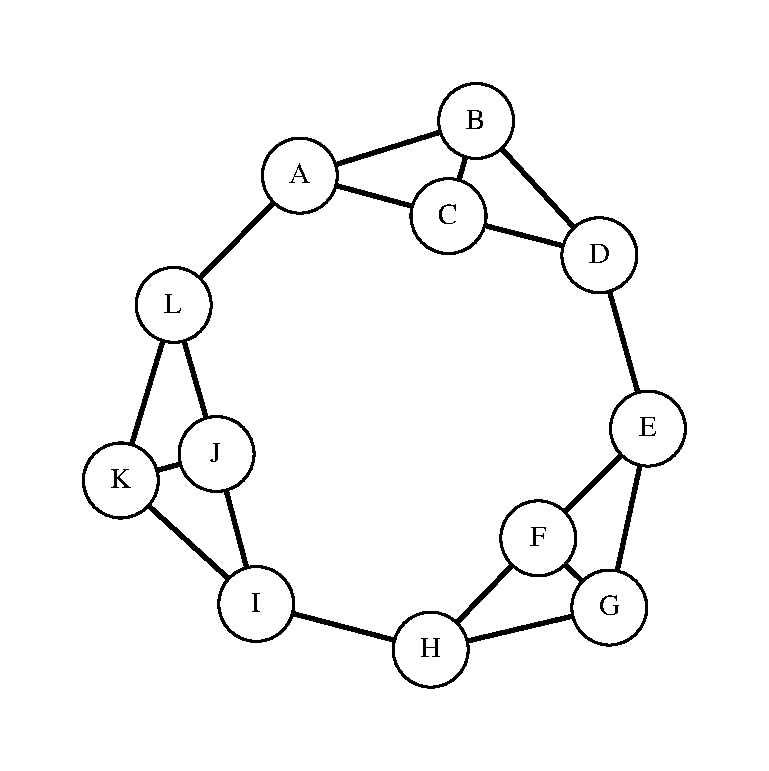
\includegraphics[scale=0.4]{graph01.pdf}
    \label{fig:graph01}
  }
  \subfloat[][Caminho na rede] {
    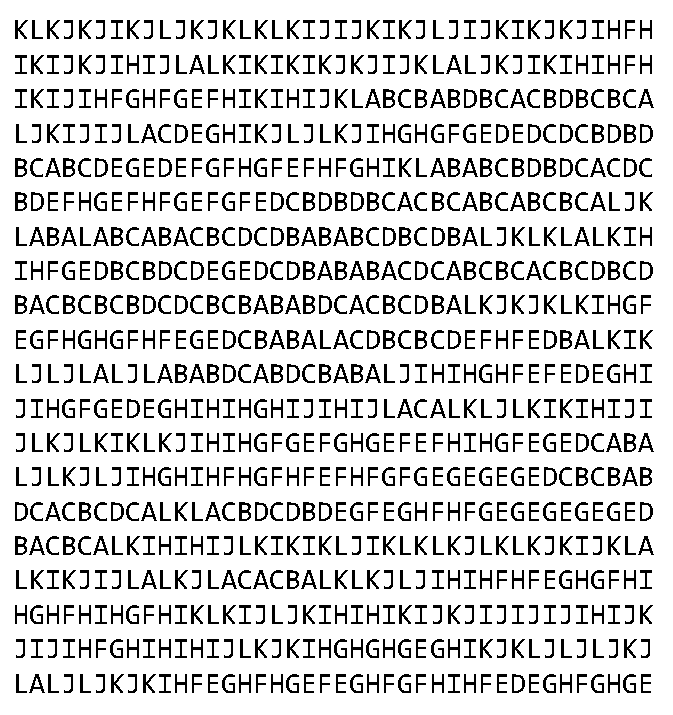
\includegraphics[scale=0.4]{graph01_path.pdf}
    \label{fig:walk01}
  }    
  \caption{Caminho de um \textit{random walker}}
\end{figure}

Apesar de ser uma rede regular, sua topologia faz com que o \textit{random walker} fique \enquote{preso} nos grupos formados pelos nós $ABCD$, $EFGH$ e $IJKL$; escapando esporadicamente de um para outro, onde circula até escapar novamente. Esses grupos são destacados na Figura~\ref{fig:graph02}. O caminho percorrido pelo \textit{walker} é exibido na Figura~\ref{fig:walk02}, dessa vez destacando os grupos por onde ele passa.

\begin{figure}[ht]
  \centering
  \subfloat[][Rede regular] {
    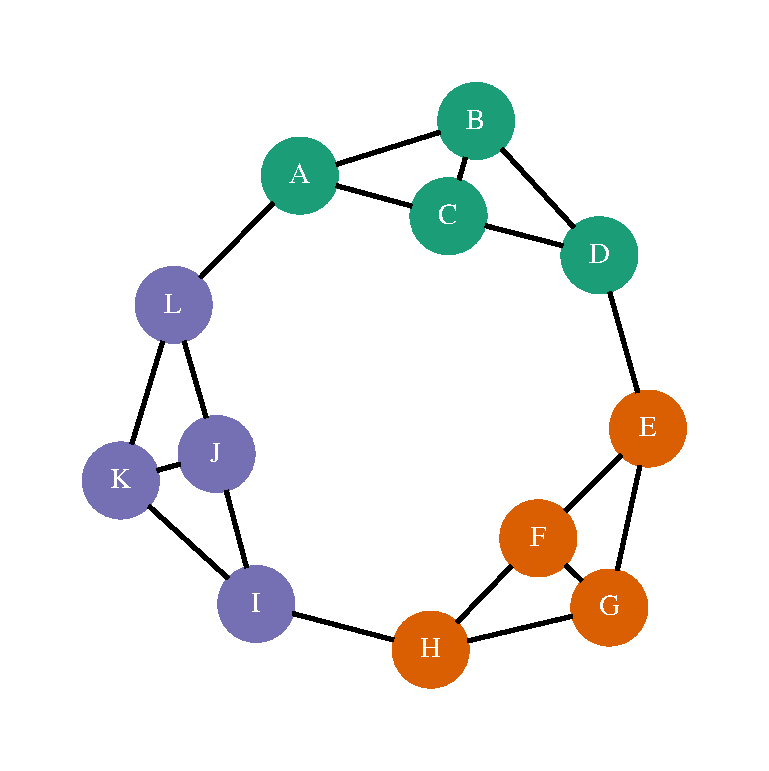
\includegraphics[width=0.4\linewidth]{graph02.pdf}
    \label{fig:graph02}
  }
  \subfloat[][Caminho no rede] {
    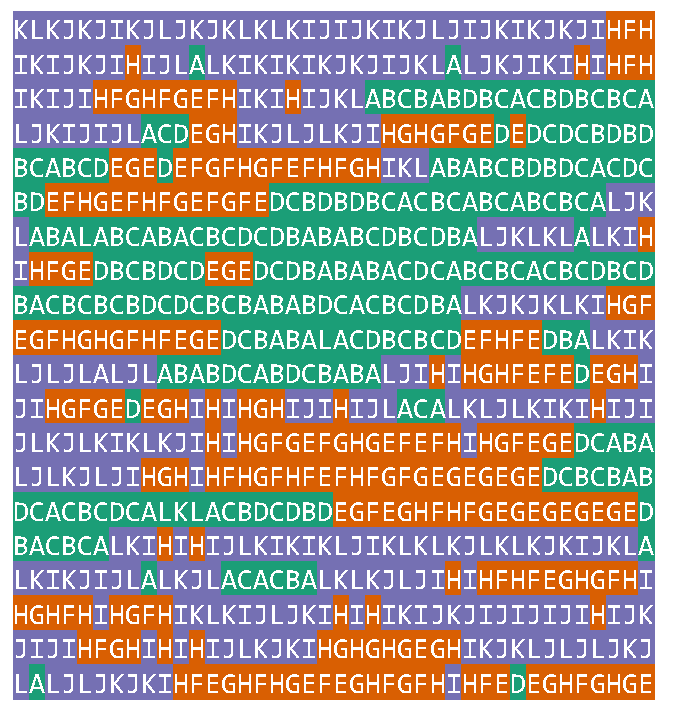
\includegraphics[width=0.4\linewidth]{graph02_path.pdf}
    \label{fig:walk02}
  }    
  \caption{Rede e caminho destacados}
\end{figure}

Se cada nó for representado por uma sequência de bits, podemos medir quanta informação é necessária para representar o caminho feito pelo \textit{random walker}. Usando a codificação de \citeonline{Huffman1952-ak} para nomear os nós de acordo com a Figura~\ref{fig:graph03}, o caminho da Figura~\ref{fig:walk01} é representado pro 2880 bits.

Se a rede for dividida em grupos como anteriormente, e usarmos uma sequência única de bits para marcar quando o \textit{walker} entra ou sai de um grupo, podemos reaproveitar os códigos usados para descrever cada nó, compactando a informação necessária para representar o caminho. A Figura~\ref{fig:graph04} mostra os códigos para a entrada de cada grupo (\enquote{0}, \enquote{10} e \enquote{11}) e os códigos de saída de cada grupo (\enquote{111}), bem como os códigos dos nós. Com essa codificação, o caminho da Figura~\ref{fig:walk01} usa 1776 bits.

\begin{figure}[ht]
  \centering
  \subfloat[][Nós usando codificação de Huffman] {
    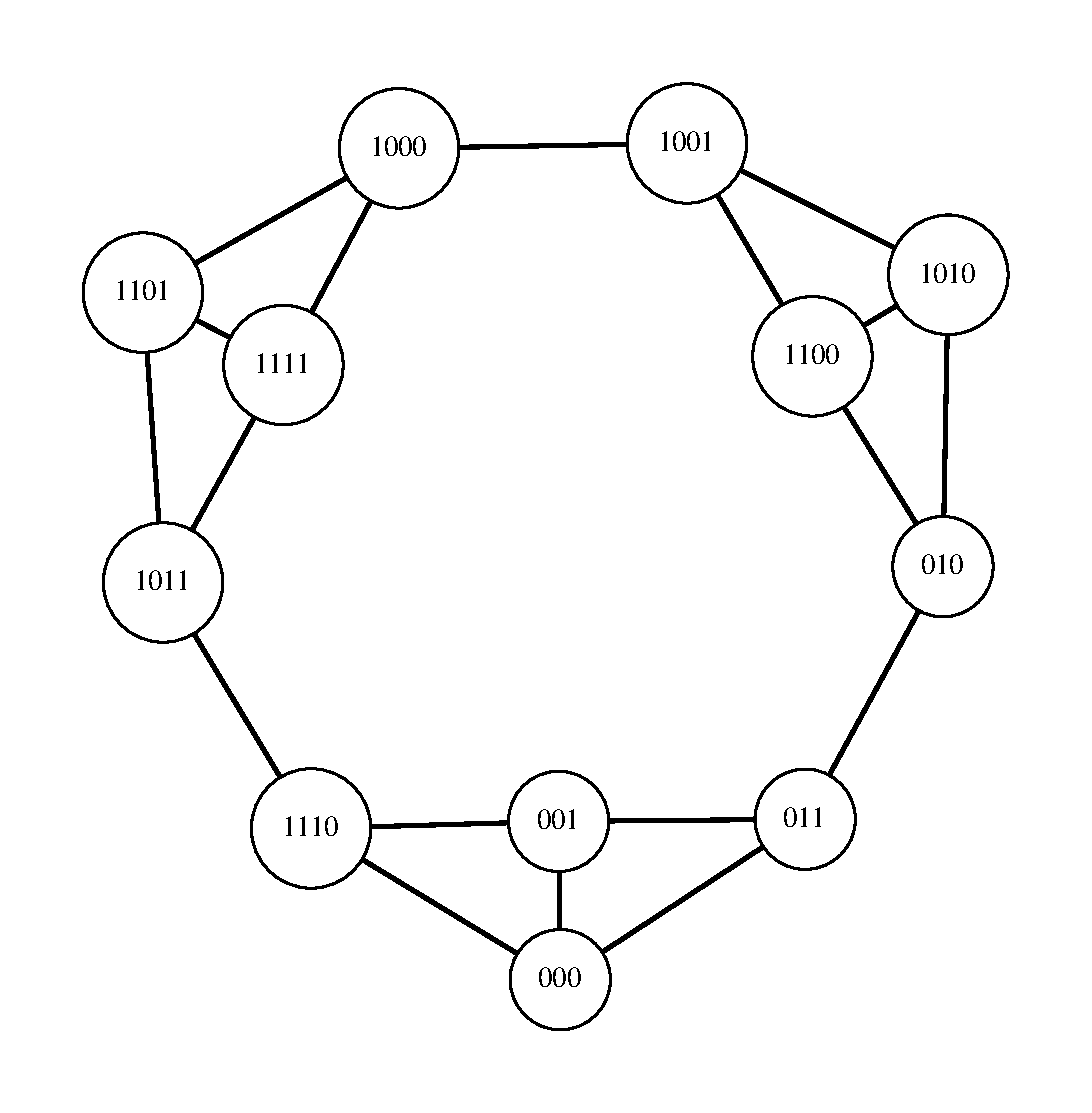
\includegraphics[width=0.4\linewidth]{graph03.pdf}
    \label{fig:graph03}
  }
  \subfloat[][Reaproveitamento de códigos] {
    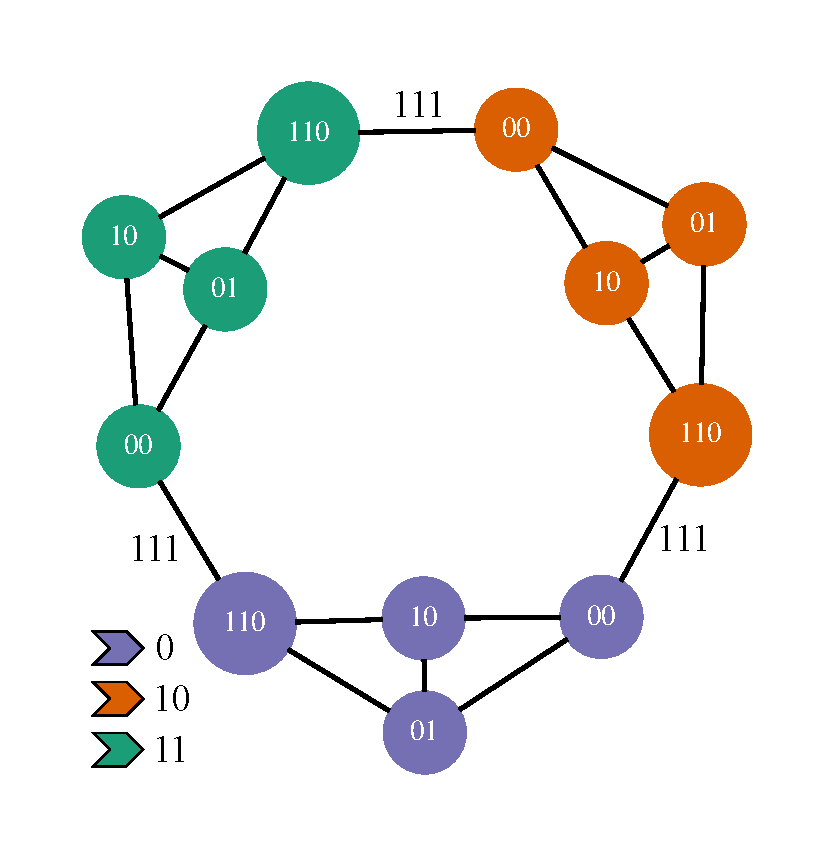
\includegraphics[width=0.4\linewidth]{graph04.pdf}
    \label{fig:graph04}
  }    
  \caption{Codificação dos nós}
\end{figure}

Portanto, o particionamento da rede em grupos onde os caminhos aleatórios podem ser representados da maneira mais compacta possível deve representar o melhor particionamento em relação ao fluxo.

A Equação de Mapa (Map Equation, \cite{Rosvall2009-sd}) permite que se identifiquem as menores codificações possíveis para uma determinado particionamento da rede sem a necessidade de se empregar \textit{random walkers} de fato. Com ela, a detecção de comunidades usando o fluxo como critério de coesão se reduz a um problema de otimização.

A Equação de Mapa é

\begin{equation*}
  L(\mathsf{M}) = q_\curvearrowright H(\mathcal{Q}) + \sum_{i=1}^{m}p^i_\circlearrowright H(\mathcal{P}^i)
\end{equation*}

Onde $L(\cdot)$ é o menor tamanho de codificação possível para representar um certo particionamento. $\mathsf{M}$ é o particionamento de $n$ nós $\alpha = 1, 2, \ldots, n$ em $m$ comunidades $i = 1, 2, \ldots, m$. O valor $q_\curvearrowright$ é a probabilidade de um \textit{random walker} sair de uma comunidade e entrar em outra. $H(\mathcal{Q})$ (\textit{eta} em maiúsculo) é a média ponderada pela frequência do comprimento dos códigos usados para entrar nas comunidades e $H(\mathcal{P}^i)$ também é a média do comprimento dos códigos ponderada pela frequência, mas dessa vez, daqueles usados na comunidade $i$. Finalmente $p^i_\circlearrowright$ é a probabilidade do \textit{walker} estar na comunidade $i$.

$H(X)$ é a equação que descreve a entropia da informação segundo uma certa distribuição de probabilidade $X$~\cite{Shannon1948-ic}. Ela se refere ao número mínimo de informação, usualmente na forma de bits, necessária para se representar uma mensagem.

A grosso modo, a Equação de Mapa pode ser descrita como: \textit{o tamanho médio dos códigos para mudança de comunidade multiplicado pela probabilidade de troca de uma por outra, somado ao tamanho médio do código de cada comunidade multiplicado pela fração de tempo que o \textit{random walker} passa em cada uma}.

Existem variações da Equação de Mapa para detecção de comunidades sobrepostas~\cite{Viamontes_Esquivel2011-it} e hierárquicas~\cite{Rosvall2011-yi}, o trabalho presente usa a variação de comunidades sobrepostas pois algumas ocupações, como \enquote{gerente de projeto} aparecem em grupos diferentes, por exemplo, relacionados a desenvolvimento de software ou a engenharia civil.


%===================================
\section{Resultados e Conclusões} \label{sec:resultados}
%===================================

A versão do MCar usada para esse trabalho possui 7.452 ocupações distintas e 90.832 conexões com ao menos 10 transições em cada uma delas.

A aplicação do algoritmo Infomap resultou em 138 comunidades \textit{não-triviais}. Uma comunidade \enquote{trivial}, nesse contexto, significa uma com apenas duas conexões, ou seja, três nós ou menos.

Em um agrupamento hierárquico, o primeiro nível possui apenas 3 grupos, um gigante composto por 6.722 nós, um segundo com 10 nós e o terceiro com 7 nós.

A existência de um grupo gigante indica de que as carreiras são bastante diversificadas, fornecendo suporte que o conceito de \textit{Carreira sem Fronteiras}.

Subdividindo o grupo gigante, encontram-se 132 grupos com tamanhos crescendo exponencialmente.

FIGURA - Grafo com a distribuição de tamanho.

O maior desses subgrupos possui em sua maioria descrições de ocupações \textit{operacionais}, indicando que não existem fronteiras claras para esses profissionais. Esse resultado aponta para a capacitação técnica como uma das maiores barreiras na movimentação profissional.

FIGURA - Exemplo de 20 ocupações do maior grupo (ilustrativo)

Cerca de X ocupações aparecem em mais de um grupo. Em sua maioria, conectam grupos com ocupações bastante distintas, indicando que são meros homônimos e não ocupações de ligação entre grupos.

FIGURA - Ocupações homônimas e outros grupos.

Muitos dos grupos menores resultam em Grafos Direcionados Acíclicos, revelando uma clara progressão de carreira. Outro são quase completamente acíclicos, com poucas conexões de pouco peso conectando nós em um aparente \enquote{retrocesso} na carreira. O significado dessas conexões é especulativo, mas uma pesquisa focada pode revelar se realmente seriam movimentos de retrocesso e suas motivações.

FIGURA - Exemplo de carreira \enquote{só pra frente}

FIGURA - Exemplo de carreira \enquote{pequena reversão}

Finalmente, o maior dos subgrupos, bem como alguns outros poucos, apresentam ciclos sem uma clara preferência. A Figura X mostra três das ocupações centrais do maior subgrupo, esse ciclo indica que algumas carreiras não são de fato uma sequência \textit{evolutiva} (em qualquer sentido possível, já que é um ciclo) como descrita por \citeonline{Arthur1989-rn}.

FIGURA X - Ciclo operacional

O aparecimento de grupos com progressão clara em oposição a grupos com a presença de ciclos fortes fornece combustível para discussões sobre modelos de carreira, em especial a noção de que \enquote{carreiras sem evolução} são comuns.

Finalmente, os próprios grupos resultantes possuem outras utilizações por si, já que representam os movimentos mais comuns nas ocupações brasileiras. Entre as possíveis aplicações eles podem ser usados como critério de classificação de ocupações; como plano de carreira baseado na progressão de menor barreira; ou como plano de treinamento de bases, já que as carreiras com progressão possuem claramente um ponto de partida; entre outros usos.

%===================================
\section{Perspectivas Futuras}
%===================================

Os resultados desse trabalho fornecem indícios que suportam modelos de carreira, como o de \textit{Carreira sem Fronteiras}, ao mesmo tempo que indicam que eles não são abrangentes para todos os segmentos profissionais. Carreiras sem Fronteiras, por exemplo, parecem ser mais apropriadas em ocupações operacionais do que para ocupações com maior exigência técnica. Análises localizadas podem comprovar ou refutar esse indício, bem como indicar quais modelos são mais adequados para quais segmentos.

Essa pesquisa contribui com suporte para um questionamento importante sobre a própria definição de carreira: que ela é um movimento \textit{evolutivo} na vida profissional de um indivíduo. A presença de ciclos fortes entre algumas ocupações sugere que existem carreiras onde não há progressão, mas sim uma movimentação lateral contante. Pesquisas orientadas podem refutar esse indício, uma vez que essa análise desconsidera os aspectos sociais e psicológicos da transição entre ocupações.

Algumas movimentações também sugerem que há retrocesso em alguns momentos da carreira. Entender se de fato são retrocessos e o que os motiva são linhas de pesquisa possíveis.

O MCar é uma fonte considerável de informação sobre o mercado de trabalho brasileiro. Outras pesquisas sobre profissões e carreira, em especial utilizando técnicas de Ciência de Redes, como \textit{motifs}, podem contribuir para uma melhor compreensão da dinâmica da movimentação profissional.

\newpage

\bibliography{main}
\end{document}
